\section{Bottlenecks}

Figure~\ref{fig:bottleneck_funnel} illustrates the main bottleneck at ElevenLabs and the strict ordering that prevents overlapping work.

\begin{figure}[H]
\centering
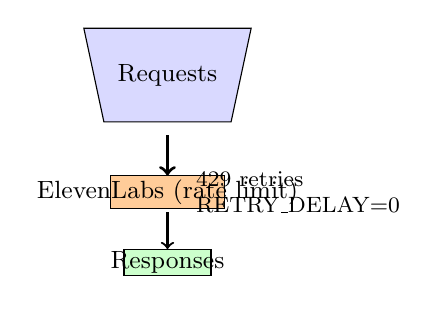
\begin{tikzpicture}[scale=0.85, every node/.style={font=\small}]
    \draw [fill=blue!15] (0,2.2) -- (2.5,2.2) -- (2.2,0.8) -- (0.3,0.8) -- cycle;
    \node at (1.25,1.5) {Requests};
    \draw [->, very thick] (1.25,0.6) -- (1.25,0);
    \draw [fill=orange!40] (0.4,0) rectangle (2.1,-0.5);
    \node at (1.25,-0.25) {ElevenLabs (rate limit)};
    \draw [->, thick] (1.25,-0.55) -- (1.25,-1.1);
    \draw [fill=green!20] (0.6,-1.1) rectangle (1.9,-1.5);
    \node at (1.25,-1.3) {Responses};
    \node [font=\footnotesize, align=left] at (3.2,-0.25) {429 retries\\RETRY\_DELAY=0};
\end{tikzpicture}
\caption[Bottleneck at TTS]{Requests are serialised at the ElevenLabs TTS layer; rate limits (HTTP 429) with zero backoff make this the primary external bottleneck.}
\label{fig:bottleneck_funnel}
\end{figure}

\begin{figure}[H]
\centering
\begin{tikzpicture}[node distance=1cm, req/.style={rectangle, draw, fill=blue!15, font=\small}, file/.style={rectangle, draw, fill=red!20, font=\footnotesize}]
    \node [req] (r1) {Request A};
    \node [req, right=2.2cm of r1] (r2) {Request B};
    \node [file, below=1.2cm of r1] (f1) {\texttt{message\_0.mp3}};
    \node [file, below=1.2cm of r2] (f2) {\texttt{message\_0.mp3}};
    \draw [->, dashed, red] (r1) -- (f1);
    \draw [->, dashed, red] (r2) -- (f2);
    \node [below=0.35cm of f1, font=\footnotesize] {same file};
    \node [below=0.35cm of f2, font=\footnotesize] {same file};
    \node [below=1.5cm of f1, font=\footnotesize, red] {concurrent writes $\Rightarrow$ overwrite};
\end{tikzpicture}
\caption[Shared filenames]{Concurrency issue: multiple requests write to the same \texttt{audios/message\_*.mp3} paths; responses can return wrong audio or phonemes.}
\label{fig:shared_filenames}
\end{figure}

\subsection{Structural Bottlenecks}
\begin{enumerate}
    \item \textbf{Single pipeline per request}: One request holds the full chain (OpenAI $\to$ lip-sync) until completion. Concurrency is limited by how many such pipelines the server runs (and by external rate limits).
    \item \textbf{ElevenLabs as bottleneck}: The code retries on HTTP 429 (rate limit) with \texttt{MAX\_RETRIES = 10} and \texttt{RETRY\_DELAY = 0}. Zero delay gives little backoff; under load, many requests can hammer the API and worsen rate limiting. ElevenLabs becomes the main external bottleneck for TTS.
    \item \textbf{Lip-sync stage ordering}: All TTS must finish before any phoneme step runs. So the slowest TTS message delays the whole phoneme phase. There is no pipeline where message 1 can already be in Rhubarb while message 2 is still in TTS.
\end{enumerate}

\subsection{Resource Bottlenecks}
\begin{enumerate}
    \item \textbf{Disk I/O}: Reads of party program, default audio/JSON, and writes of \texttt{audios/message\_*.mp3}, \texttt{*.wav}, \texttt{*.json}. Under concurrency, multiple requests can contend on the same \texttt{audios} directory (and overwrite \texttt{message\_0.mp3} etc.\ if not isolated per request).
    \item \textbf{Process spawning}: Each request runs multiple ffmpeg and Rhubarb processes. No process pool or queue; under load this can stress the OS and CPU.
    \item \textbf{Memory}: Base64-encoded audio and full JSON are held in memory per message and returned in one response; large replies increase memory and response size.
\end{enumerate}

\subsection{Correctness and Robustness}
\begin{itemize}
    \item \textbf{Shared filenames}: \texttt{audios/message\_0.mp3}, \texttt{message\_1.mp3}, etc., are shared across requests. Concurrent requests can overwrite each other’s files and return wrong audio or phonemes. This is a critical correctness bottleneck.
    \item \textbf{Error handling}: If TTS or Rhubarb fails for one message, the error is logged and an empty \texttt{mouthCues} is used; the rest of the pipeline continues. Whisper or OpenAI failures fall back to default or “I didn’t catch that” without retry or cost control.
\end{itemize}
